\section{Mathematical formulation of SHE}\label{Section2}

This section is devoted to the mathematical formulation of the SHE problem. In what follows, with the notation $\mathcal U$ we will always refer to a finite set of real numbers, contained in the interval $[-1,1]$
\begin{align}\label{eq:Udef}
	\mathcal U = \{u_\ell\}_{\ell=1}^L\subset [-1,1],
\end{align}
with cardinality $|\mathcal U| = L$. 

In broad terms, our objective is to design a piece-wise constant function $u(\tau):[0,2\pi)\to\mathcal U$ such that some of its lower-order Fourier coefficients take specific values determined a priori. 

 
\begin{figure}
	\centering
	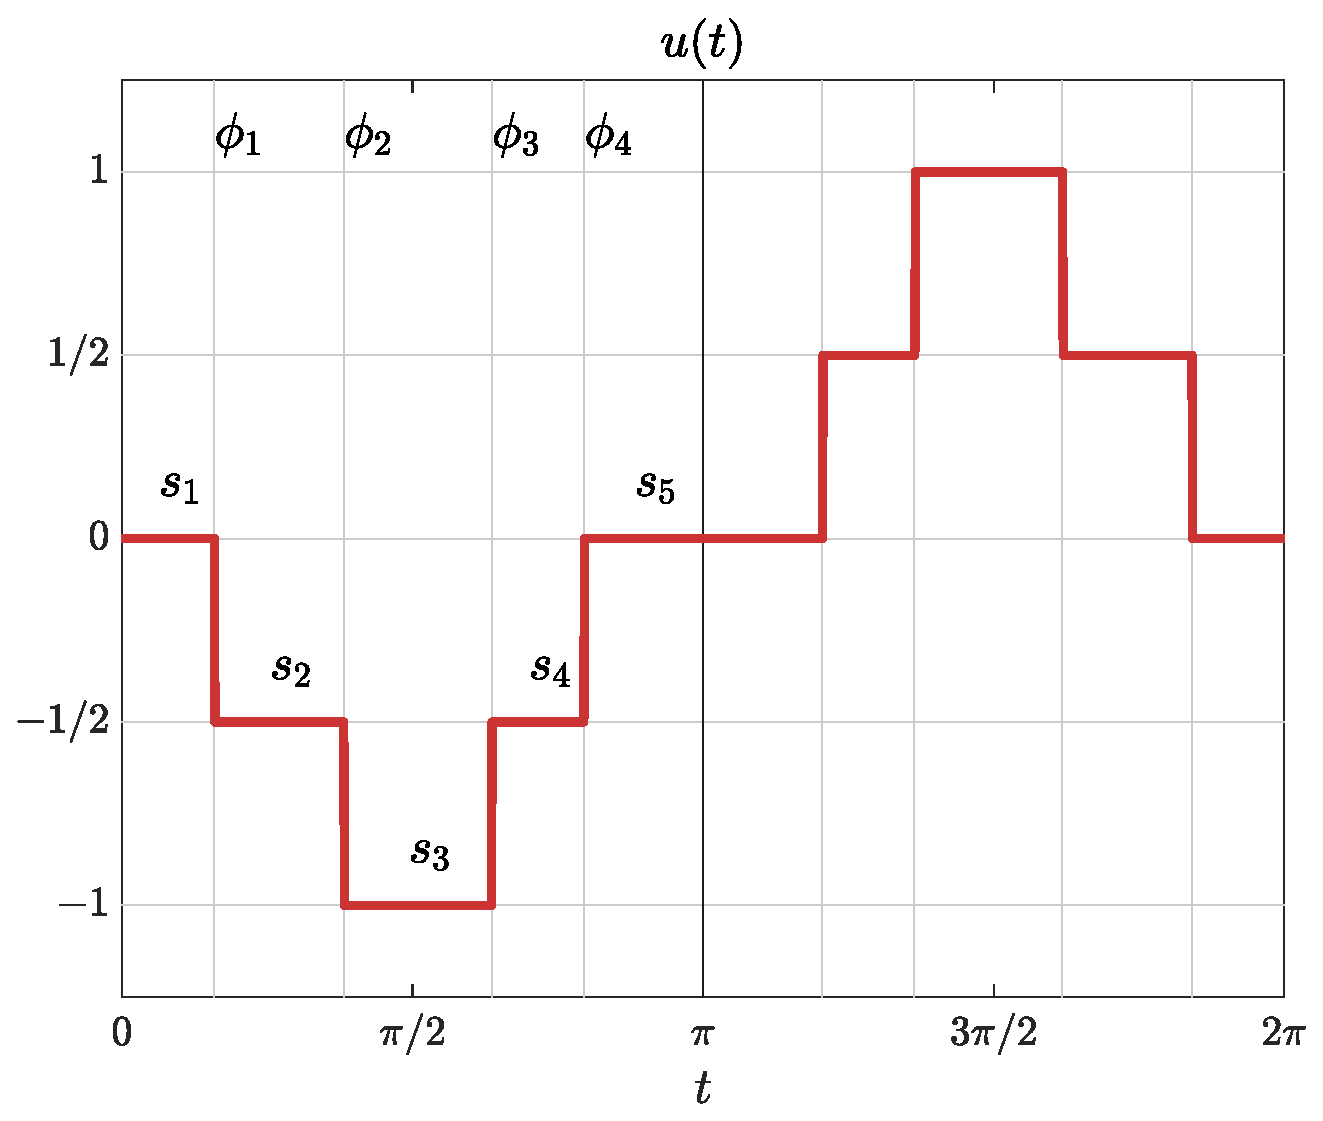
\includegraphics[scale=0.35]{img/fig01.eps} 
	\caption{A Step function and possible solution of Problem \ref{pb:SHEp}, where we considered a possible finite set of control $\mathcal{U} = \{-1/3, -2/3, 0, 1/3, 2/3, 1\}$. We show the switching angles $\bm{\phi}$ and the waveform $\mathcal{S}$ (see Definitions \ref{def:waveform} and \ref{def:switchingAngles}). \textcolor{red}{tengo que darle la vuelta en el tiempo}}\label{fig:exampleSHE}
\end{figure}

Due to the application in power converters, we will focus here on functions with \textit{half-wave symmetry}, i.e. 
\begin{align*}
	u(\tau + \pi) = -u(\tau)\quad \mbox{for all}\; \tau \in [0,\pi).
\end{align*}
In this way, $u$ is fully determined by its values in the interval $[0,\pi)$ and its Fourier series only involves the odd terms, thus taking the form
\begin{equation}
	u(\tau ) = \sum_{\underset{i\, odd}{i \in \mathbb{N}}} a_i \cos(i\tau)+ \sum_{\underset{j\, odd}{j \in \mathbb{N}}}  b_j \sin(j \tau), 
\end{equation}
where the coefficients $a_i$ and $b_j$ are given by
\begin{equation} \label{eq:an}
	\begin{aligned}
		a_i = \frac{2}{\pi} \int_0^\pi u(\tau ) \cos(i \tau)\,d\tau, 
		\\
		b_j = \frac{2}{\pi} \int_0^\pi u(\tau)  \sin(j \tau)\,d\tau.
	\end{aligned}
\end{equation}
Because of this half-wave symmetry, in what follows, we will always work with the restriction $u|_{[0,\pi)}$ which, with some abuse of notation, we shall still denote by $u$. We can then give a general formulation of the SHE problem as follows:
\newline
\begin{problem}[SHE]\label{pb:SHEp}
Let $\mathcal{E} _a $ and $\mathcal{E} _b $ be two sets of odd numbers with cardinalities $|\mathcal{E}_a| = N_a $ and $ |\mathcal{E} _b| = N_b$, respectively, and $\mathcal{U}$ be defined as in \eqref{eq:Udef}. Given the vectors $\bm{a}_T \in \mathbb{R}^{N_a}$ and $\bm{b}_T \in \mathbb{R}^{N_b} $, we look for a piece-wise constant function $u: [0,\pi)\to\mathcal{U}$ such that 
\begin{gather}
	\notag a_i = (\bm{a}_T)_i, \quad\textrm{ for all } i \in \mathcal{E}_a,
	\\
	\notag b_j = (\bm {b}_T)_j, \quad\textrm{ for all } j \in \mathcal{E}_b,
\end{gather}
with $\{a_i\}_{i\in\mathcal E_a}$ and $\{b_j\}_{j\in\mathcal E_b}$ given by \eqref{eq:an}.
\end{problem} 
 
Fig. \ref{fig:exampleSHE} shows an example of a function $u$ solution of the SHE problem. 

